% \chapter{Theoretical Backgound}
\chapter{Fundamente teoretice}
În acest capitol se vor prezenta fundamentele teoretice proiectului, și se vor explica în detaliu deciziile architecturale luate în elaborarea proiectului.\newline
Scopul proiectului a fost proiectarea și implementarea unui program/sistem care este capabil să clasifice obiecte din imagini, să poată face detecția obictelor (adică să specifice unde se află acestea în imagine) și să facă segmentarea semantică a imaginii. Am ajuns la decizia că pentru aceste probleme o să folosesc o rețea neuronală convoluțională deoarece rețelele neuronale depășesc orice altă abordare capabilă să efectueze aceste sarcini.\newline
În primul rând o să se facă prezentarea rețelelor neuronale (convoluționale) și straturile specifice acestora. După aceasta vom afla cum se întâmplă antrenarea rețelei.

\section{Rețele Neuronale Convoluționale}
O rețea neuronală convoluțională - ca orice rețea neuronală - are la bază conceptul de \textit{neuron}, acesta fiind elementul din care se construiește. Aceștia sunt organizați în \textit{straturi de neuroni} (layer), straturile fiind interconectate formând o \textit{ierarhie de straturi}.\newline
Informația de intrare este alimentată \textit{stratului de intrare} (input layer). După aceasta semnaul se propagă printr-o serie de \textit{straturi ascunse}; în fiecare strat neuronii își calculează activarea prin folosirea \textit{funcției de activare}, iar activările se propagă în direcția \textit{stratului de ieșire} (output layer). Stratul de ieșire la rândul lui va furniza informația necesară (e.g. clasificarea obiectului din imagine, detecția obiectelor, segmentarea semantică, etc.).

\subsection{Neuronul Artificial}
În contextul științei biologiei neuronul este o celulă, un bloc de construcție, a cărui rol este colectarea semnalelor de la neuronii vecini prin dentriți, procesarea acestor informații, și pe baza informațiilor obținute și a structurii interne emite un semnal al lui prin axonul lui.\newline
%image of biological neuron
\begin{figure}[h!]
    	\centering
	\captionsetup{justification=centering, margin=2cm}
	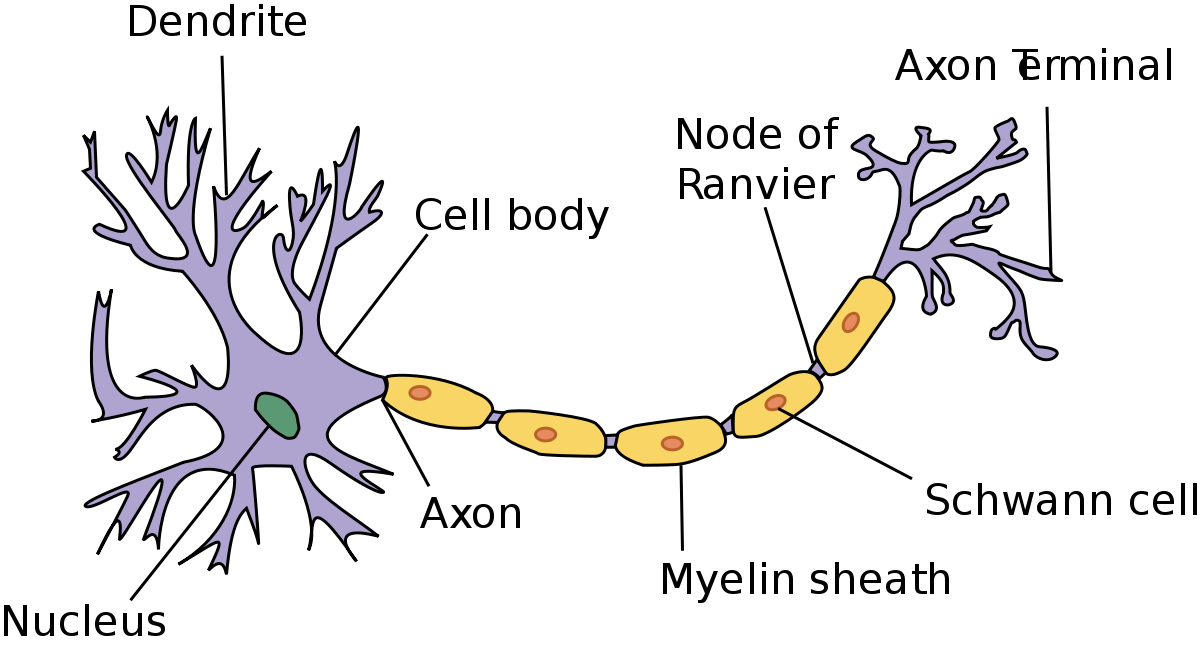
\includegraphics[width=0.5\textwidth]{figures/neuron.png}
	\caption{Neuronul - blocul de construcție a sistemului nervos \cite{neuron}}
	\label{fig:segmentare_semantica}
\end{figure}
Ideea neuronului artificial este bazată pe aceeași idee, părțile din care se compune fiind:
\begin{itemize}
	\item Intrările ponderate: semnalele/activările stratului anterior în șir sunt ponderate, asta însemnând că un neuron poate fi mai mult sau mai puțin influențat de un alt neuron. Ponderile sunt învățate în faza antrenării rețelei. Prin ponderi se introduce conceptul de \textit{neurons that fire together wire together}.
	\item Funcție de activare: pe baza intrărilor se calculează cât de tare este activat acest neuron.
	\item Ieșire: semnalul de activare se propagă la neuronii din stratul următor prin ieșirea lui.
\end{itemize}
%image of biological neuron
\begin{figure}[h!]
    	\centering
	\captionsetup{justification=centering, margin=2cm}
	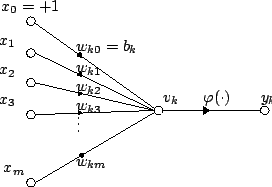
\includegraphics[width=0.5\textwidth]{figures/an.png}
	\caption{Modelul neuronului artificial \cite{arn}}
	\label{fig:neuronul_artificial}
\end{figure}

Dacă ne uităm la funcțiile de transfer a neuronilor artificiali des folosite, vedem că există mai multe tipuri sau categorii de neuroni acestea fiind:

\begin{itemize}
	\item \textit{Threshlod neurons} (neuronii cu funcția treaptă): acest tip de neuron are cea mai simplă funcție de activare; ia intrările de la neuronii din stratul anterior, multiplică activările acestora cu ponderea respectivă pentru fiecare și calculează suma numerelor obținute după înmulțire. Înainte de a da ai departe rezultatul, se mai scade un număr special, numit \textit{bias}. Dacă rezultatul scăderii este mai mare decât zero, atunci ieșirea neuronului este unu, altfel 0.
	\item \textit{Linear combination neuron} (neuronii cu funcția de transfer liniară - purelin): acest tip de neuron se comportă asemănător cu neuronii de prag. Ia intrările, calculează suma intrărilor ponderate și din această sumă scade bias-ul. Dacă rezultatul este mai mic decât zero, atunci activarea acestui neuron va fi zero. Între zero și unu, se propagă mai departe valoarea calculată. Peste unu, valoarea trimisă mai departe va fi și ea unu.
	\item \textit{Sigmoid neuron}:  neuronii care fac parte din această categorie folosessc o funcție non-liniară pentru a calcula activările lor: funcția sigmoidală. Această funcție este aleasă fiindcă calcularea derivativei ei este ușoară aceasta fiind a caracteristică crucială pentru a face posibilă antrenarea rețelei cu ajutorul algoritmului \textit{baskpropagation}.
\begin{equation}
	f(z) = \frac{1}{1 + \mathrm{e}^{-z}}
\end{equation}
unde
\begin{equation}
	z = b + x_1w_1 +  x_2w_2 + \dots + + x_nw_n
\end{equation}
\end{itemize}

%image of biological neuron
\begin{figure}[h!]
    	\centering
	\captionsetup{justification=centering, margin=2cm}
	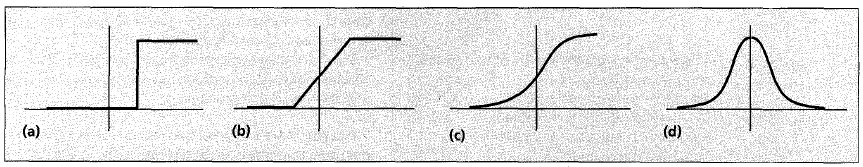
\includegraphics[width=0.5\textwidth]{figures/activation_functions.png}
	\caption{Funcții de transfer \cite{activationFunctions}}
	\label{fig:activationFunctions}
\end{figure}


\subsection{Rețeaua Neuronală Artificială}
Acum că am stabilit ce este un neuron artificial, categoriile neuronilor și funcționarea fiecăruia, putem lua un pas înapoi să vedem imaginea întreagă: rețeaua neuronală artificială care este construită din neuroni.\newline
Rețelele neuronale artificiale sunt utilizate pe scală largă în contextul inteligenței artificiale. Modelul și modul de funcționare a acestora este inspirată de modelul rețelelor neuronale din sistemul nervos al animalelor și al omului (imitând funcționarea sistemului nervos central sau a creierului).\newline
Popularitatea lor provine din faptul că acestea sunt capabile de a învăța funcți incredibil de complexe, cu mii de parametri (datoritp numărului mare de ponderi care pot fi învățate pentru a ajunge la o estimare cu ajustare precisă). Rețelel neuronale au urmâtoarele caracteristici importante:
\begin{itemize}
	\item Architectură: aceasta cuprinde decizii asupra numărului de straturi de neuroni, parametrii ca și numărul neuronilor pe fiecare strat aparte, ponderile conexiunilor, și inițializarea acestora.
	\item Regula de învățare/algoritmul de învățare: este mechanismul ales care va îndeplini sarcina ajustării ponderilor în fiecare iterație de antrenare. Alegerea algoritmului corespunzător este de o importanță crucială, și trebuie examinată pentru că un algoritm necorespunzător ar putea rezulta în incapabiliatea de a antrena rețeaua.
	\item Funcțiile de transfer a neuronilor din fiecare strat
\end{itemize}
Rețelele neuronale au o serie de straturi de neuroni, acestea de obicei fiind numerotate de la $L_0$ până la $L_N-1$ unde N este adâncimea rețelei neuronale. Neuronii de pe stratul $L_i$ primesc intrările de la stratul anterior, $L_i-1$. Folosind aceste intrări neuronul aplică funcția lui de transfer, rezultatul fiin activarea neuronului. Această activare se propagă mai departe spre stratul următor, adică $L_i+1$ unde va constitui parte din intrările neuronilor.
\begin{figure}[h!]
    	\centering
	\captionsetup{justification=centering, margin=2cm}
	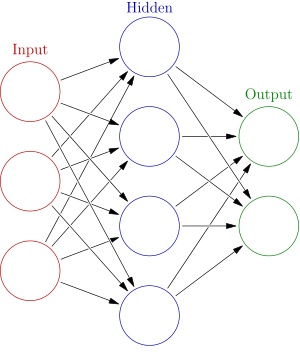
\includegraphics[width=0.5\textwidth]{figures/artificialneunet_1hidden.png}
	\caption{Funcții de transfer \cite{arn}}
	\label{fig:activationFunctions}
\end{figure}





\label{cap:fund-teoretice}

Aici se descriu pe scurt aspecte teoretice pe care se bazează lucrarea. Conținutul acestui capitol trebuie gândit pentru un citor care nu e specializat pe domeniul temei și nu cunoaște chestiunile de bază despre subiect. Pentru un cititor specializat, capitolul poate să stabilească un limbaj comun, relativ la termenii care pot fi interpretați diferit. 

Acest capitol nu trebuie gândit și scris nici ca un copy-paste din alte surse, nici ca zona de reglaj a numărului de pagini ale lucrării. Deși va conține chestiuni pe care le-ați studiat și voi și pe care v-ați bazat, el trebuie să fie o compilare a surselor folosite, care să aibă sens și relevanță pentru lucrarea voastră. Trebuie să fie o descriere coerentă și logică a unor aspecte care ușurează sau fac posibilă înțelegerea părților următoare ale lucrării. Nu trebuie intrat insă prea mult în detalii, ci spuse doar chestiunile esențiale. 

Dacă preluați text, figuri, tabela etc. din sursele de documentare, acestea din urmă trebuie indicate explicit. 

Reprezintă cca. 10\% din lucrare.